% Noctra Whitepaper: Public and Private Lending on Horizen
% Build: latexmk -pdf noctra-whitepaper_v2.tex  (or pdflatex, bibtex, pdflatex, pdflatex)
\documentclass[11pt,a4paper]{article}

\usepackage[T1]{fontenc}
\usepackage[utf8]{inputenc}
\usepackage{lmodern}
\usepackage[margin=2.5cm]{geometry}
\usepackage{amsmath,amssymb}
\usepackage{booktabs}
\usepackage{tabularx}
\usepackage{array}
\usepackage{enumitem}
\usepackage[dvipsnames]{xcolor}
\usepackage{tikz}
\usetikzlibrary{arrows.meta,positioning,shapes.geometric,fit,backgrounds,calc}
\usepackage{caption}
\captionsetup[figure]{position=top}
\captionsetup[table]{position=top}
\usepackage[numbers]{natbib}
\usepackage[hidelinks]{hyperref}
\usepackage{microtype}
\usepackage{placeins}

\newcolumntype{L}{>{\raggedright\arraybackslash}X}
\setlist{itemsep=2pt,topsep=4pt}

\definecolor{nborder}{HTML}{8A8A80}
\definecolor{naccent}{HTML}{1F6FD6}
\definecolor{ngood}{HTML}{1E9E3A}
\definecolor{nzone}{HTML}{F2F1EC}

\tikzset{
  box/.style={draw=nborder, rounded corners=3pt, align=center, minimum width=3.6cm,
              minimum height=1.1cm, font=\small, line width=0.6pt},
  accent/.style={box, draw=naccent, fill=naccent!10, line width=1.2pt},
  dec/.style={diamond, draw=nborder, aspect=2.2, align=center, font=\small,
              inner sep=1pt, line width=0.6pt},
  arr/.style={-{Stealth[length=2mm]}, draw=nborder, line width=0.7pt},
  lbl/.style={font=\footnotesize\color{black!65}},
  zone/.style={draw=nborder!60, fill=nzone, rounded corners=4pt, inner sep=8pt},
}

\newcommand{\code}[1]{\texttt{#1}}

\title{\textbf{Noctra}\\[4pt]\large Public and Private Lending on Horizen}
\author{Henk-Wim de Boer\\Blockstat Solutions}
\date{Draft v2 --- 28 September 2026}

\begin{document}
\maketitle

\begin{abstract}
\noindent Noctra is a lending protocol on Horizen, an OP Stack L3 on Base, that will offer public and private
borrowing and lending from one shared pool of liquidity. The public version is built: an Aave-style pool for
WETH and USDC with interest indices, a kinked rate model, health-factor liquidations and a Chainlink price feed
relayed from Base by a $k$-of-$n$ set of relayers. The pool and oracle are covered by unit, fuzz and invariant
tests and an internal security review.

The private version hides who owns a position, how large it is and what its owner does with it, while pool
totals stay public so solvency remains verifiable. Private positions exist on-chain only as commitments with
encrypted data, funds move through a shielded token pool, private actions are settled in batches per epoch so
the public totals do not reveal individual actions, and a trusted execution environment (TEE) computes health
factors on hidden data. A position is revealed only at the moment it becomes liquidatable, backed by a ZK proof
that it really is, so permissionless keepers can still liquidate it; a protocol vault acts as a fallback. The
design rule is that a broken TEE may leak data but can never move funds: every private state change, including
a liquidation, is checked on-chain by a ZK proof.

Noctra builds directly on ZKPerp, the author's prize-winning private perpetuals exchange on Aleo (top three at
the Aleo $\times$ AKINDO Buildathon). It reuses ZKPerp's tooling and patterns: a Chainlink price relay with a
relayer quorum, off-chain liquidation bots, a Merkle-allowlist compliance layer and viewing keys, together with
its lessons on liquidation under privacy. Perpetual trading on Horizen is the planned next product,
sharing Noctra's oracle, collateral and privacy layer.
\end{abstract}

\tableofcontents
\newpage

% ---------------------------------------------------------------------------
\section{Introduction and motivation}

On a public chain, every loan is an open book: anyone can see who borrowed, how much, against what, and at
which price the position will be liquidated. For individuals that is a privacy problem. For businesses, funds
and treasuries it is a commercial one, because size and leverage are exactly what competitors and
counterparties want to know.

Public loans also create a specific market risk. Because every liquidation price is visible, a large position
can be targeted: on a chain with thin liquidity it can pay to push the price just past that level and collect
the liquidation bonus. Hiding amounts removes the map that makes this attack easy.

Horizen is a natural home for this. It relaunched as an OP Stack L3 on Base in December 2025 with a focus on
regulatory-compliant privacy~\citep{theblock2025}. The chain itself is public; privacy lives at the application
layer~\citep{horizen2026,horizenprivacy}, with Horizen Labs tooling such as Vela, a confidential execution
service running in AWS Nitro Enclaves~\citep{veladocs}, and zkVerify for proof verification~\citep{zkverify}. Noctra uses that split: a public lending core, and a private layer on top of
the same liquidity.

Offering both from one pool matters on a new chain. Two separate pools would split already thin liquidity,
raise rates on both sides and make liquidations less reliable. With one pool, public and private users earn and
pay the same rates and share the same depth.

\paragraph{Built on ZKPerp.} Noctra is not a first attempt. It uses the same tools and patterns as
ZKPerp~\citep{zkperp}, a privacy-preserving perpetuals exchange on Aleo by the same author, live on Aleo
testnet:
\begin{itemize}
  \item \textbf{Oracle relay.} Chainlink prices read on another chain and relayed by a quorum of independent
        relayers, checked on-chain (2-of-3 in ZKPerp, $k$-of-$n$ in Noctra).
  \item \textbf{Off-chain services.} A relayer backend and permissionless liquidation bots that watch positions
        and act when they fail.
  \item \textbf{Compliance.} A Merkle allowlist for entry screening and viewing keys for selective disclosure.
\end{itemize}
Section~\ref{sec:zkperp} compares the two designs in detail. ZKPerp's whitepaper~\citep{zkperp}, source
code~\citep{zkperpcode} and live app~\citep{zkperpapp} are public:
\begin{itemize}[itemsep=0pt]
  \item Whitepaper: \url{https://hwdeboer1977.github.io/ZKPerp/zkperp-whitepaper-v5.html}
  \item Code: \url{https://github.com/hwdeboer1977/ZKPerp}
  \item App: \url{https://zk-perp.vercel.app/}
\end{itemize}

% ---------------------------------------------------------------------------
\clearpage
\section{Architecture overview}

Noctra v1 has three parts: Chainlink prices on Base, off-chain relayers and liquidators, and two contracts on
Horizen (Figure~\ref{fig:arch}). Horizen has no native Chainlink feeds, so prices are read on Base and relayed.

\begin{figure}[!ht]
\centering
\caption{Noctra v1 architecture: prices flow from Chainlink on Base to the pool on Horizen.}
\label{fig:arch}
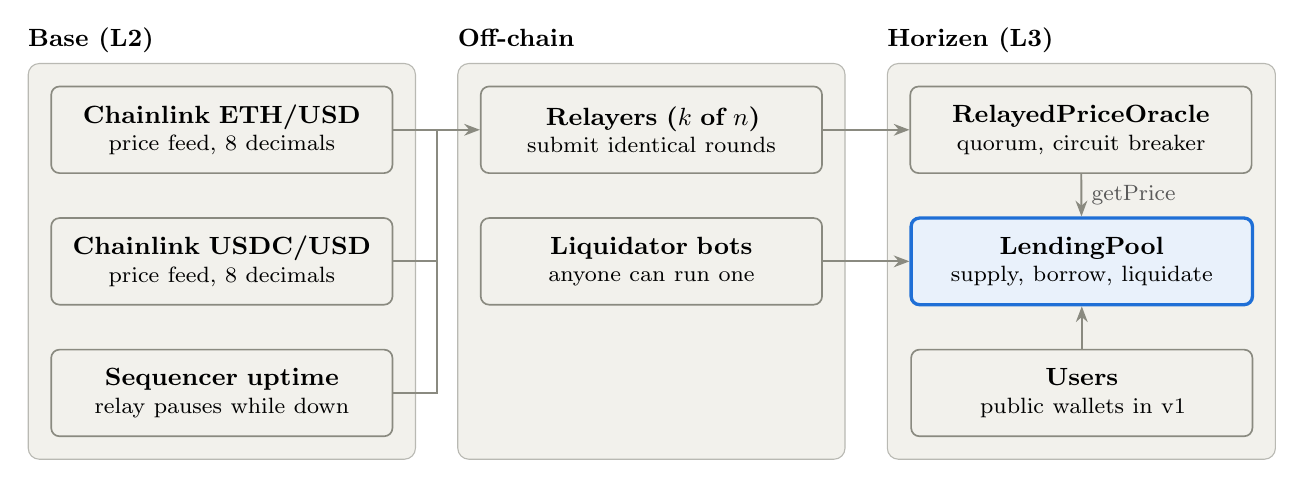
\begin{tikzpicture}[node distance=0.55cm and 1.1cm,
    fbox/.style={box, text width=4.1cm},
    zlabel/.style={font=\small\bfseries, anchor=base west, inner sep=0pt, yshift=6pt}]
  % Base column
  \node[fbox] (eth)  {\textbf{Chainlink ETH/USD}\\[-1pt]{\footnotesize price feed, 8 decimals}};
  \node[fbox, below=of eth] (usdc) {\textbf{Chainlink USDC/USD}\\[-1pt]{\footnotesize price feed, 8 decimals}};
  \node[fbox, below=of usdc] (seq) {\textbf{Sequencer uptime}\\[-1pt]{\footnotesize relay pauses while down}};
  % Off-chain column
  \node[fbox, right=of eth] (rel) {\textbf{Relayers ($k$ of $n$)}\\[-1pt]{\footnotesize submit identical rounds}};
  \node[fbox, right=of usdc] (liq) {\textbf{Liquidator bots}\\[-1pt]{\footnotesize anyone can run one}};
  % Horizen column
  \node[fbox, right=of rel] (orc) {\textbf{RelayedPriceOracle}\\[-1pt]{\footnotesize quorum, circuit breaker}};
  \node[accent, text width=4.1cm, right=of liq] (pool) {\textbf{LendingPool}\\[-1pt]{\footnotesize supply, borrow, liquidate}};
  \node[fbox] (users) at (seq -| pool) {\textbf{Users}\\[-1pt]{\footnotesize public wallets in v1}};

  \begin{scope}[on background layer]
    \node[zone, fit=(eth)(seq)] (zbase) {};
    \node[zone, fit=(rel)(seq.south -| liq)] (zoff) {};
    \node[zone, fit=(orc)(users)] (zhor) {};
  \end{scope}
  \node[zlabel] at (zbase.north west) {Base (L2)};
  \node[zlabel] at (zoff.west |- zbase.north) {Off-chain};
  \node[zlabel] at (zhor.west |- zbase.north) {Horizen (L3)};

  % the three Base readings merge on one bus into the relayers
  \coordinate (bus) at ($(eth.east)!0.5!(rel.west)$);
  \draw[draw=nborder, line width=0.7pt] (usdc.east) -- (usdc.east -| bus);
  \draw[draw=nborder, line width=0.7pt] (seq.east) -- (seq.east -| bus) -- (bus);
  \draw[arr] (eth.east) -- (rel.west);
  \draw[arr] (rel) -- (orc);
  \draw[arr] (liq) -- (pool);
  \draw[arr] (orc) -- node[lbl, right] {getPrice} (pool);
  \draw[arr] (users) -- (pool);
\end{tikzpicture}
\end{figure}

Relayers read the same Chainlink round and submit it to \code{RelayedPriceOracle}; a price counts once $k$ of
$n$ agree. The pool reads prices through the \code{IPriceOracle} interface, so the oracle can be swapped
without changing the pool. Liquidator bots scan borrowers and liquidate positions below a health factor of 1.
A read-only price server exposes the same Base readings over HTTP for monitoring.

% ---------------------------------------------------------------------------
\section{The public lending pool (v1)}

The v1 pool is a single Solidity contract that lets users supply WETH and USDC, borrow against them, repay with
interest and be liquidated. It follows the Aave design~\citep{aavev3} closely, without its complexity.

\subsection{Interest and rounding}

Each asset has two indices that start at 1.0 (in RAY, $10^{27}$): a liquidity index for what suppliers earn and
a borrow index for what borrowers owe. Users store scaled balances, and their real balance is always the scaled
balance times the current index:
\begin{equation}
  \text{balance}(t) = \text{scaled} \cdot \text{index}(t), \qquad
  \text{scaled} = \frac{\text{amount}}{\text{index}(t_0)} .
\end{equation}
Every action first accrues the indices for the time elapsed, so interest reaches every user without looping
over them. The interest added to total debt is credited to suppliers and, for the reserve factor, to the
treasury, so the books stay balanced up to a few wei of rounding. This is an accounting property: it counts all
debt as an asset, including bad debt that can no longer be collected (Section~\ref{sec:gaps}).

Every conversion between amounts and scaled balances rounds in the pool's favour: suppliers get slightly less
claim, borrowers owe slightly more. A full exit burns the whole scaled balance, so no dust is left behind.

\subsection{Kinked rate model}

The borrow rate depends on utilization $U = \text{debt} / (\text{cash} + \text{debt})$. It rises slowly up to
an optimal utilization $U^*$ and steeply above it, which pulls utilization back and keeps withdrawals possible:
\begin{equation}
  r_b =
  \begin{cases}
    r_0 + s_1 \dfrac{U}{U^*} & U \le U^* \\[8pt]
    r_0 + s_1 + s_2 \dfrac{U - U^*}{1 - U^*} & U > U^*
  \end{cases}
  \qquad
  r_s = r_b \cdot U \cdot (1 - \rho) .
\end{equation}
Here $\rho$ is the reserve factor: the share of interest that goes to the treasury as a supply position.
Utilization uses cash tracked inside the pool, not the token balance, so donating tokens cannot push rates
down. Table~\ref{tab:rates} lists the launch parameters.

\begin{table}[h]
\centering
\caption{Rate model parameters.}
\label{tab:rates}
\begin{tabular}{lrrrrr}
\toprule
Asset & Base rate $r_0$ & Slope $s_1$ & Kink $U^*$ & Slope $s_2$ & Reserve factor $\rho$ \\
\midrule
WETH & 0\% & 3\% & 80\% & 80\% & 15\% \\
USDC & 0\% & 4\% & 90\% & 60\% & 10\% \\
\bottomrule
\end{tabular}
\end{table}

% ---------------------------------------------------------------------------
\section{Risk parameters and liquidations}

Each collateral asset has two ratios: a loan-to-value (LTV) that caps how much a user may borrow, and a higher
liquidation threshold (LT) that decides when a position can be liquidated. The gap between them is a buffer, so
a position opened at maximum LTV is not liquidatable in the same block.

\begin{table}[h]
\centering
\caption{Risk parameters.}
\label{tab:risk}
\begin{tabular}{lrrr}
\toprule
Asset & LTV & Liquidation threshold & Liquidation bonus \\
\midrule
WETH & 75\% & 80\% & 7.5\% \\
USDC & 70\% & 75\% & 5\% \\
\bottomrule
\end{tabular}
\end{table}

These are more conservative than Aave on Ethereum mainnet, on purpose: Horizen's DEX liquidity is thinner, so
liquidators need a larger bonus and more room to sell seized collateral.

\subsection{Health factor and liquidation}

A position's health factor is
\begin{equation}
  HF = \frac{\sum_i \text{collateral}_i \cdot \text{price}_i \cdot LT_i}{\sum_j \text{debt}_j \cdot \text{price}_j}
\end{equation}

At $HF \ge 1$ a position is safe; below 1 anyone may liquidate it. The contract enforces
$LTV \le LT < 100\%$ and $LT \cdot (1 + \text{bonus}) < 100\%$ for every asset. Without the second rule, the
collateral a liquidator is owed at $HF = 1$ would exceed what exists, and every liquidation would create bad
debt.

A liquidator repays part of the debt and receives collateral worth that amount plus the bonus. Above
$HF = 0.95$ at most 50\% of the debt can be repaid per call (the close factor); below 0.95 the whole debt can be
closed. If the collateral cannot cover the bonus, the liquidator takes all of it and covers proportionally less
debt.

\subsection{Worked example}

Bob supplies 1 WETH at \$3{,}000 and borrows the maximum 2{,}250 USDC (75\% LTV). His health factor is
$3{,}000 \times 0.80 / 2{,}250 = 1.067$.
\begin{enumerate}
  \item ETH falls to \$2{,}750. $HF = 2{,}200 / 2{,}250 = 0.978$, so Bob is liquidatable. The liquidation price
        was $2{,}250 / 0.80 = \$2{,}812.50$.
  \item $HF$ is above 0.95, so a liquidator may repay at most 1{,}125 USDC.
  \item The liquidator receives $1{,}125 \times 1.075 / 2{,}750 = 0.4398$ WETH, worth \$1{,}209.38: a profit of
        \$84.38 before gas.
  \item Bob keeps 0.5602 WETH against 1{,}125 USDC of debt. His health factor rises to 1.096, so he is safe
        again.
\end{enumerate}

% ---------------------------------------------------------------------------
\section{Price oracle}

\code{RelayedPriceOracle} accepts a Chainlink~\citep{chainlink} price on Horizen once $k$ of $n$ relayers have
submitted exactly the same round from Base. Every honest relayer reads the same data (round id, answer, update
time), so an exact match is required and no median is needed.

\begin{description}[style=nextline, leftmargin=1.5em, font=\normalfont\bfseries]
  \item[Vote key.] Each vote is keyed by the relayer-set epoch, the asset and the full round. Changing relayers
        or the quorum starts a new epoch, so old votes never count toward a new set.
  \item[Sanity checks.] A round must have a positive answer, no future timestamp beyond 60 seconds of drift,
        and be strictly newer than the last known round. Malformed or replayed data reverts.
  \item[Staleness.] \code{getPrice} reverts when Chainlink's own update time is older than the asset's maximum
        age: about 70 minutes for ETH and 25 hours for USDC, each just above the feed's heartbeat.
  \item[Circuit breaker.] A round that moves the price more than the allowed deviation (20\% for ETH, 50\% for
        USDC) trips the asset instead of being accepted. \code{getPrice} then reverts immediately, and the owner
        either accepts the new price or discards it. The pool stops using the old price at once rather than
        keeping it alive until it goes stale.
\end{description}

The relayer backend skips ticks while the Base sequencer is down or within an hour of restarting, and simulates
each submission before sending it.

\paragraph{Trust model.} The oracle cannot see Base. It trusts that at least $k$ relayers are honest, so relayer
keys run on separate infrastructure and the owner is a multisig. A later version could replace relayers with
storage proofs against Base's block hash.

% ---------------------------------------------------------------------------
\section{Testing and security status}

The pool and the oracle are tested in three layers (78 tests in total, plus 7 invariants), have had an internal
security review, and are not yet externally audited or deployed to Horizen testnet.

\begin{table}[h]
\centering
\caption{Test layers.}
\begin{tabularx}{\textwidth}{@{}p{3.2cm}L@{}}
\toprule
Layer & What it covers \\
\midrule
Pool unit tests (40) & Admin checks, supply and withdraw, borrowing at and above LTV, a year of interest
  accrual, rate-model changes, liquidation at 50\% and 100\% close factor, bad debt after a crash \\ \addlinespace
Oracle unit tests (27) & Quorum and exact-match voting, decimal scaling, replay and older-round rejection,
  circuit breaker tripping, accepting and resetting, staleness measured from Chainlink's time, relayer
  removal and quorum limits, a USDC depeg within the loose breaker \\ \addlinespace
Mock tests (11) & Mock ERC-20 and mock oracle used in tests and the demo \\ \addlinespace
Fuzz tests & Liquidation accounting at any price and amount; solvency after random borrow, repay and time
  jumps \\ \addlinespace
Invariant tests (7) & Random sequences of all actions, prices and time jumps across 4 users. After every call:
  cash equals token balance, scaled balances sum to totals, cash plus debt covers supply, indices never
  decrease, no borrow beyond LTV, every liquidation reduces debt and collateral, utilization at most 100\% \\ \addlinespace
End-to-end demo & Deploy on a local anvil node, drop the ETH price, liquidate with the backend bot \\
\bottomrule
\end{tabularx}
\end{table}

The invariant suite found one real bug: once the borrow index exceeds 1, a liquidation repaying 1 wei burned
zero scaled debt while still seizing collateral. The pool now rejects such a liquidation, with a regression
test.

\paragraph{Known gaps before mainnet.}\label{sec:gaps}
\begin{itemize}
  \item \textbf{Bad debt.} Debt left without collateral cannot be cleared and keeps accruing interest, which
        inflates supplier and treasury claims. A write-off mechanism is next on the roadmap.
  \item \textbf{Oracle outages.} When a price is stale or the breaker trips, liquidations stop for affected
        users, exactly when prices move most.
  \item \textbf{Admin powers.} Oracle and risk parameters change instantly; a timelock is needed.
  \item \textbf{Missing controls.} No supply or borrow caps, no emergency pause and no minimum borrow size yet.
  \item \textbf{Zero-threshold collateral.} An asset with a liquidation threshold of 0 can still be seized, and
        its bonus is not capped.
\end{itemize}

% ---------------------------------------------------------------------------
\section{Private lending: goals and threat model}

The private side hides who owns a position, how large it is, and what its owner does with it, while keeping
liquidations open and the pool verifiably solvent. It does not make users invisible. On a public chain, money
entering and leaving a privacy system is always visible. The goal is \emph{unlinkability}: an observer who sees
Alice deposit cannot tell what she did afterwards, or which later withdrawal is hers.

\subsection{The privacy model}
\label{sec:privmodel}

Noctra's privacy rests on three rules.
\begin{description}[leftmargin=0pt, labelsep=0.5em]
  \item[Aggregates are public.] Total supply, total debt, cash and utilization per asset stay public. Rates are
        computed from them, anyone can verify that the pool is solvent, and the pool's token balance is public on
        Horizen anyway. Like Zcash's turnstile, public totals also make it detectable if a bug ever creates value
        out of nothing.
  \item[Positions are private.] The owner, size, collateral and debt of each private position are hidden. Only
        commitments and encrypted data appear on-chain.
  \item[Changes are batched.] If private actions settled one by one, each change to the public totals would
        reveal the size of one action. Private actions are therefore collected per epoch and settled as one net
        change. The public sees how much private borrowing rose in an epoch, not who borrowed or how much.
\end{description}
Entry and exit sit outside these rules. A deposit into the shielded pool shows the depositor's address and
amount; a withdrawal shows the amount and destination. Privacy covers everything in between.

\subsection{Levels of privacy}

\begin{table}[h]
\centering
\caption{Levels of privacy.}
\small
\begin{tabularx}{\textwidth}{@{}>{\raggedright\arraybackslash}p{2.3cm}LLLL@{}}
\toprule
Level & Hidden & Stays public & Liquidation & Trust \\
\midrule
1. Unlinkable & Owner & Size, health factor, liquidation price & Anyone computes $HF$ & Math only \\
\addlinespace
2. Confidential \textbf{(Noctra)} & Owner, size, link between actions & Totals, net change per epoch, entry and
  exit & Enclave reveals a position once $HF<1$ & TEE for confidentiality, ZK proofs for integrity \\
\addlinespace
3. Hidden aggregates \textit{(ruled out)} & Also totals and utilization & Only entry and exit & Same as
  level 2 & TEE or committee; solvency unverifiable \\
\bottomrule
\end{tabularx}
\end{table}

\textbf{Level 1} hides only the owner. A large position can often be identified by its size, and its public
liquidation price still invites the price attack described in Section~1.

\textbf{Level 2} is Noctra's choice. It hides everything that identifies or exposes a user, while keeping public
what the pool needs: totals for rates and solvency. Batched settlement (Section~\ref{sec:privmodel}) stops those
totals from revealing individual actions.

\textbf{Level 3} is listed only for comparison: it is neither possible nor desirable. The pool's cash is a
public token balance, rates reveal utilization, and hiding totals would make solvency unverifiable.

\subsection{What is hidden, and what still leaks}

\paragraph{Who we hide from.}
\begin{itemize}
  \item \textbf{The public and chain analysts:} owner and size are hidden.
  \item \textbf{Competitors and counterparties:} position size and leverage are hidden.
  \item \textbf{Liquidation hunters:} liquidation prices are never published in advance.
  \item \textbf{The protocol team:} does not see positions; there is no operator viewing key for liquidations.
        If the team also operates the enclave hardware, this rests on the TEE's confidentiality holding
        against its own operator, which is exactly what a TEE is meant to provide but not something the
        chain can enforce.
  \item \textbf{An auditor or regulator:} can see what the compliance design allows (Section~\ref{sec:compliance}).
  \item \textbf{Anyone watching entry and exit:} can see deposits into and withdrawals from the shielded pool, but
        not link them to each other or to activity inside.
\end{itemize}

\paragraph{What still leaks.}
\begin{itemize}
  \item \textbf{Entry and exit.} Every deposit into and withdrawal from the shielded pool shows an address and an
        amount. Withdrawing to the same address as the deposit reconnects the two.
  \item \textbf{Net change per epoch.} Each epoch's net change in private supply and debt is public. With few
        private users, it can reveal a single action.
  \item \textbf{Timing and amount patterns.} A deposit of 4,987.31 followed by an epoch whose net change is
        exactly 4,987.31 identifies the user. Round amounts and waiting help.
  \item \textbf{Liquidations.} A liquidated position's size becomes public at that moment, not its owner.
  \item \textbf{Network metadata.} IP addresses, RPC providers and frontends can link actions off-chain.
  \item \textbf{Privileged views.} The enclave sees all private state by design, and an auditor sees what the
        compliance design allows.
  \item \textbf{Past data after a key compromise.} Ciphertexts encrypted to the enclave's key stay on-chain
        forever. Whoever extracts that key can decrypt every private position ever stored under it, not only
        current ones. Rotating the key protects positions re-encrypted after the rotation, but cannot un-publish
        old ciphertexts. A TEE breach is therefore a permanent, retroactive loss of privacy for everything
        stored under the leaked key, even though it cannot move funds.
\end{itemize}

\paragraph{Privacy is a crowd property.} Cryptography hides values, but unlinkability depends on how many others use the system at the same time. One
private borrower in an epoch has no cover, however strong the proofs. Privacy on Noctra will therefore be weak at
launch and strengthen with usage. Longer epochs give more cover but slower settlement. Users improve their own
privacy by using common amounts, waiting between entry and use, and exiting to a different identity than they
entered with.

% ---------------------------------------------------------------------------
\section{Private architecture}

Public and private positions live in the same pool, keyed by a position identifier instead of an address.
Interest, health factors and liquidation logic operate on positions, so they stay the same for both.

\begin{table}[h]
\centering
\caption{Public and private positions in the same pool.}
\begin{tabularx}{\textwidth}{@{}p{3cm}LL@{}}
\toprule
 & Public position & Private position \\
\midrule
Position id & Hash of the owner's address & Commitment to the owner's public key and the position state \\ \addlinespace
Authorization & Transaction sender & ZK proof of the owner's spending key, with a nullifier against replay \\ \addlinespace
Balances on-chain & Plain & A commitment plus encrypted data (Section~\ref{sec:privpos}) \\ \addlinespace
Funds in and out & Directly from and to a wallet & Through a shielded token pool \\ \addlinespace
Gas & Paid by the user & Paid through a relayer \\ \addlinespace
Health factor & Computed by anyone & Proven by the owner for their own actions; monitored by the TEE for
  liquidation \\ \addlinespace
Settlement & Immediately & Per epoch, netted with other private actions \\
\bottomrule
\end{tabularx}
\end{table}

\subsection{The private position}
\label{sec:privpos}

A private position is isolated: one collateral asset and one debt asset. This keeps each position's state small
and its health factor simple to prove. Its state is committed on-chain as
\[
  C = H(\mathit{pk}_{\mathit{own}},\ \mathit{collAsset},\ \mathit{scaledColl},\ \mathit{debtAsset},\
  \mathit{scaledDebt},\ \mathit{nonce}).
\]
Collateral and debt are stored as scaled balances, like public positions, so interest accrues through the
indices without the commitment changing. The nonce makes every commitment unique.

As in Zcash, the owner's keys are split by what they allow. The \emph{spending key}, from which
$\mathit{pk}_{\mathit{own}}$ is derived, authorizes the owner's own actions and never leaves the owner. The
\emph{viewing data} (the opening of $C$ and the nullifier key) lets its holder read the position and prove
statements about it, but not act for the owner. The enclave receives the viewing data only. It can therefore
prove that a position is liquidatable, but it cannot borrow, withdraw or move collateral on the owner's behalf.

Next to each commitment, two ciphertexts of the same state are stored on-chain: one encrypted to the enclave's
key and one to the owner's key. The first lets the enclave monitor health factors. The second makes
the owner independent of the enclave: if it goes offline, the owner can still read their state and exit through
the escape hatch.

Positions are updated UTXO-style. Every action spends the current commitment by publishing its nullifier and
creates a new commitment. A nullifier cannot be linked to the commitment it spends, so observers cannot tell
whether two actions concern the same position. Table~\ref{tab:where} summarizes where each piece of data lives.

\begin{table}[h]
\centering
\caption{Where private position data lives.}
\label{tab:where}
\begin{tabularx}{\textwidth}{@{}p{3.6cm}L@{}}
\toprule
Location & What it holds \\
\midrule
On-chain, public & Commitments, nullifiers, ciphertexts, per-asset totals, oracle prices, epoch net changes \\ \addlinespace
Inside the enclave & Decrypted position states and viewing data, health factors; never spending keys \\ \addlinespace
With the user & Spending key, position opening and nonce, their own decryption key \\ \addlinespace
Visible to the public & No owner, no collateral amount, no debt amount, no link between actions \\
\bottomrule
\end{tabularx}
\end{table}

\subsection{Four mechanisms, four jobs}
\label{sec:mechanisms}

\begin{description}[leftmargin=0pt, labelsep=0.5em]
  \item[Commitments give integrity.] The contract and ZK proofs check against them. They reveal nothing about the
        values inside.
  \item[Ciphertexts give availability.] They keep private state recoverable without trusting any single party to
        store it.
  \item[ZK proofs give correctness.] Each state change proves that the new commitment follows from the old one
        under the protocol's rules, without revealing values. For the owner's own actions the owner generates
        the proof: they know their state and want the action to go through, so they prove for example that a
        borrow stays within LTV. For a liquidation, the enclave generates a proof that the position's health
        factor is below 1. Either way, the contract verifies the proof, which is what stops a compromised
        enclave from forging state or triggering false liquidations.
  \item[The TEE gives hidden monitoring.] The enclave holds the decryption key for private positions and
        recomputes health factors when prices change. It adds what none of the others can: it evaluates hidden
        state when nobody has an incentive to prove it. A borrower never wants to prove they are underwater,
        so the enclave does it for them.
\end{description}
Noctra plans to use Vela~\citep{veladocs} as its TEE. Vela runs application logic in AWS Nitro Enclaves; the
enclave's identity is established by hardware attestation, and every result it returns is signed by the attested
enclave and verified on-chain. Vela is at v0.2.0 on Base Sepolia and Horizen testnet, with mainnet on its
roadmap. Two properties shape Noctra's design. First, the enclave has no external networking, so it cannot read
prices or chain state itself: its host must feed it. A malicious host can withhold or delay that input, but
cannot make a healthy position liquidatable, because the liquidation proof is checked against the prices and
indices stored on-chain. Second, trusting the enclave means trusting AWS's Nitro hardware and attestation, which
is one more reason integrity must not depend on it.

Keeping the TEE out of ordinary actions is deliberate. The less the enclave has to do, the smaller the damage
if it is compromised or offline: users can still act on their own positions with their own proofs.

The central rule is that \emph{a compromised TEE may leak data but must never drain the pool}. TEEs have a long
record of side-channel attacks, so confidentiality is treated as breakable. Integrity must not rest on the
enclave:
\begin{itemize}
  \item The authoritative state stays on-chain as commitments; the enclave only proposes state changes.
  \item The contract enforces conservation: debt only falls with a repayment, collateral only moves with a
        matching burn, and totals must reconcile.
  \item Each private state change carries a ZK proof that the contract verifies, so a forged change is rejected
        even if the enclave is compromised.
  \item This includes liquidations. A liquidation instruction is accepted only with a proof that the committed
        position has a health factor below 1 at the oracle price and indices on-chain. An enclave attestation
        alone is not enough: otherwise a compromised enclave could declare a healthy position liquidatable and
        hand its collateral, plus the bonus, to a keeper.
\end{itemize}
Until the proof system is in place, integrity rests partly on the enclave, including the decision that a position
is liquidatable, and private deposits should be capped accordingly.

\subsection{Moving funds and settling in batches}
\label{sec:batch}

The shielded token pool holds tokens as private notes: commitments to an amount and an owner secret. Depositing
creates a note and is public (address and amount). Inside the pool, notes can be split, merged and transferred to
other users privately, using nullifiers as above.

The shielded pool and the lending pool are deliberately separate steps. A user first deposits into the shielded
pool and later, in a separate action, uses a note to supply collateral. If deposits went straight into a
position, the depositor's address would be attached to that position from the start. Borrowed funds likewise
arrive as a new note in the shielded pool, not in a wallet.

A relayer submits private transactions and pays their gas, so no user address appears as the sender. The same
shielded pool can later fund other private applications on Horizen, such as private perpetuals, so notes can
circulate without ever touching a public address.

Private actions are collected per epoch of $E$ blocks and settled together at its end. The pool accrues interest
once, applies the net change in private supply, debt and cash, and moves the net token amount between the
shielded pool and the lending pool in one transfer. Borrows and repays within an epoch cancel out in the public
totals.

LTV checks for private actions use the price and indices at settlement, and the new commitments and nullifiers
are finalized then. The cost is latency: a private borrow is available at the end of its epoch, not immediately.

Because the owner generates the proof before settlement, it cannot use the settlement price directly. Instead,
the proof takes a worst-case bound as public input: a minimum collateral price and a maximum borrow index, and
shows that the action stays within LTV at those bounds. At settlement the contract accepts the action only if
the actual price and index are within the bounds. The owner chooses how much margin to leave; a wider margin is
less likely to fail but allows a smaller borrow.

\paragraph{When a private action fails at settlement.} Two cases must be handled explicitly:
\begin{itemize}
  \item \textbf{The market moved.} If the settlement price or index falls outside an action's bounds, that
        action is dropped. Its nullifier is not recorded, so the old commitment stays valid and the owner can
        resubmit with a new proof. Nothing is lost except the epoch's wait.
  \item \textbf{Not enough cash.} If the epoch's net private borrowing and withdrawals exceed the pool's cash,
        actions are settled in submission order until cash runs out, and the rest are dropped in the same way.
        Public borrows during the epoch can use up cash too; a private user sees the same liquidity risk as a
        public one, only later.
\end{itemize}
Dropped actions are visible only as a count, not as amounts or owners.

\subsection{Example: Alice borrows privately}

\begin{enumerate}
  \item Alice deposits 5,000 USDC from her wallet into the shielded pool. \emph{Public: her address, 5,000.}
  \item Later, through the relayer, she uses the note to open a private position. \emph{Public: a nullifier and a
        new commitment.}
  \item She requests a 2,000 USDC borrow with a ZK proof that she owns the position and that the borrow stays
        within LTV at her chosen price bound. No enclave is involved.
  \item At the end of the epoch, private borrowing is netted and settled. \emph{Public: the epoch's net change in
        debt.}
  \item Alice receives a 2,000 USDC note in the shielded pool. She can repay, pay others privately, or withdraw.
\end{enumerate}
If she withdraws 2,000 to her original address, an observer sees 5,000 go in and 2,000 come out, but cannot tell
whether that was a loan, a partial withdrawal or a payment she received. Withdrawing to an unrelated address
removes even that link.

\paragraph{Refactor first.} The first step is a pure refactor of the v1 pool from address-keyed to position-keyed storage, with no privacy
yet. All existing unit, fuzz and invariant tests must still pass, which makes the change verifiable before any
private logic is added.

% ---------------------------------------------------------------------------
\section{Liquidation under privacy}

A private position is revealed only when it becomes liquidatable, and only its liquidation terms. Pure ZK cannot
do this: a borrower has no incentive to prove they are underwater, so someone must be able to evaluate hidden
health factors. In Noctra that is the TEE (Figure~\ref{fig:liq}). The TEE decides \emph{when} to act; a ZK
proof decides \emph{whether} the action is valid.

\begin{figure}[h]
\centering
\caption{Private liquidation flow: positions stay hidden until they become liquidatable.}
\label{fig:liq}
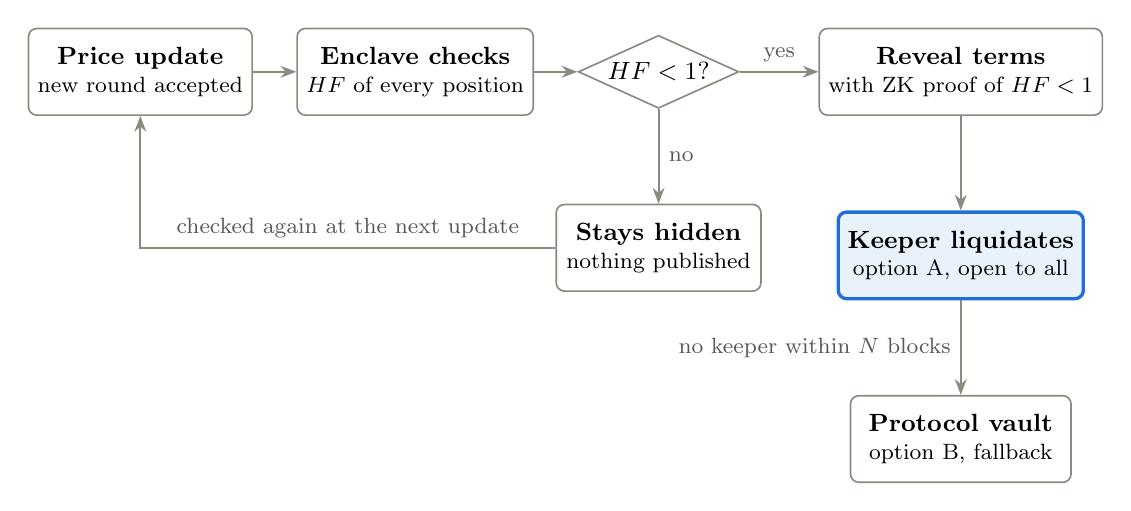
\begin{tikzpicture}[node distance=0.8cm and 0.55cm]
  \node[box, minimum width=2.6cm] (price) {\textbf{Price update}\\[-1pt]{\footnotesize new round accepted}};
  \node[box, minimum width=2.8cm, right=of price] (encl) {\textbf{Enclave checks}\\[-1pt]{\footnotesize $HF$ of every position}};
  \node[dec, right=of encl] (hf) {$HF < 1$?};
  \node[box, minimum width=2.8cm, right=1.0cm of hf] (rev) {\textbf{Reveal terms}\\[-1pt]{\footnotesize with ZK proof of $HF<1$}};
  \node[box, minimum width=2.6cm, below=1.2cm of hf] (hide) {\textbf{Stays hidden}\\[-1pt]{\footnotesize nothing published}};
  \node[accent, minimum width=2.8cm, below=1.2cm of rev] (keep) {\textbf{Keeper liquidates}\\[-1pt]{\footnotesize option A, open to all}};
  \node[box, minimum width=2.8cm, below=1.2cm of keep] (vault) {\textbf{Protocol vault}\\[-1pt]{\footnotesize option B, fallback}};

  \draw[arr] (price) -- (encl);
  \draw[arr] (encl) -- (hf);
  \draw[arr] (hf) -- node[lbl, above] {yes} (rev);
  \draw[arr] (hf) -- node[lbl, right] {no} (hide);
  \draw[arr] (rev) -- (keep);
  \draw[arr] (keep) -- node[lbl, left] {no keeper within $N$ blocks} (vault);
  \draw[arr] (hide.west) -| node[lbl, above, pos=0.25] {checked again at the next update} (price.south);
\end{tikzpicture}
\end{figure}

\paragraph{Option A: reveal on liquidation (default).} After each price update the enclave checks every private
position. For a position below $HF = 1$ it publishes an instruction (the position's nullifier, the debt to
repay and the collateral to seize) together with a ZK proof that the committed position has $HF < 1$ at the
current on-chain price and indices and that the terms follow the protocol's close factor and bonus. The
contract verifies the proof; an instruction without a valid proof is rejected, whoever signed it. Any keeper can
then execute it with their own capital, as in the public pool. Healthy positions and their liquidation prices
are never published.

\paragraph{Option B: protocol vault (fallback).} If no keeper acts within $N$ blocks, a protocol vault executes
the same instruction. The vault needs no viewing key; it acts only on an instruction whose proof the contract
has verified. Its capital source, rewards and loss handling are still to be designed.

Seeing and executing are split. The enclave sees; keepers or the vault execute; the protocol team holds no
viewing key for liquidations.

\paragraph{Escape hatch.} If the enclave stops sending heartbeats for a set period, the pool enters escape mode.
Users read their state from their own ciphertext and act with their own proofs, so funds stay reachable if the
TEE operator disappears:
\begin{itemize}
  \item \textbf{New borrows stop.} Nobody is watching health factors, so no new risk is taken on.
  \item \textbf{Repay and withdraw stay open.} A user can repay debt from shielded notes and withdraw collateral,
        or withdraw part of their collateral with a proof that $HF \ge 1$ still holds at the current oracle
        price. A user with debt cannot simply walk away with their collateral.
  \item \textbf{Liquidations stop.} Without the enclave nobody can see which positions fail. Positions that go
        underwater during the outage can turn into bad debt, the same failure mode as an oracle outage in the
        public pool. The private deposit cap bounds that loss, and the bad-debt write-off from the hardening
        phase absorbs it.
\end{itemize}

% ---------------------------------------------------------------------------
\section{Relation to ZKPerp and the path to perpetuals}
\label{sec:zkperp}

Noctra's private design builds on ZKPerp~\citep{zkperp}, a privacy-preserving perpetuals exchange on Aleo by the
same author. It runs on Aleo testnet, with a mainnet pilot in preparation. Its source code~\citep{zkperpcode} and live app~\citep{zkperpapp} are
public.

ZKPerp combines a GMX-style pooled counterparty vault, a concentrated-liquidity AMM and a ZK dark pool with
uniform-price batch auctions. Its oracle is relayed by a quorum of relayers, liquidations are run by a race
between keepers, and a compliance layer gates trading with a Merkle allowlist.

\begin{table}[h]
\centering
\caption{What carries over from ZKPerp.}
\begin{tabularx}{\textwidth}{@{}p{3.2cm}LL@{}}
\toprule
Topic & ZKPerp on Aleo & Noctra on Horizen \\
\midrule
Privacy base & Native: Aleo records are private by default & Application layer: the chain is public, so a TEE
  plus ZK proofs \\
Who can see positions for liquidation & Protocol keepers and operator & Only the enclave; keepers see a
  position only once it is liquidatable \\
Oracle & Relayed prices with a quorum & Chainlink on Base, relayed with a $k$-of-$n$ exact-match quorum \\
Compliance & Merkle allowlist, operator viewing key & Same pattern, with an auditor viewing key \\
Off-chain services & Oracle relayers, liquidation bot, compliance server & Oracle relayers and liquidator bots;
  compliance service planned \\
\bottomrule
\end{tabularx}
\end{table}

The main lesson from ZKPerp is that liquidation is the hardest part of private DeFi: someone must be able to see
enough to act when a position fails. Noctra's answer separates seeing (the enclave) from executing (open
keepers), which ZKPerp could not do on Aleo alone.

\paragraph{Perpetuals on Horizen.} Private perpetual trading is the planned next product. It would reuse Noctra's relayed oracle, its TEE-based
privacy layer and the same liquidation design. Two further links are worth evaluating: using collateral
supplied to Noctra as trading margin, and whether a perps liquidity vault could serve as the lending pool's
liquidation backstop. The second couples the two products' risks, so it needs its own analysis before any
decision.

% ---------------------------------------------------------------------------
\section{Compliance design}
\label{sec:compliance}

Noctra aims for privacy from the public, not from lawful oversight. That matches Horizen's positioning, which
offers view keys and access logs so applications can tailor privacy levels~\citep{horizenroadmap}.

\begin{itemize}
  \item \textbf{Entry screening.} Deposits into the shielded token pool can be restricted to an allowlist,
        following ZKPerp's Merkle-allowlist pattern, or to Privacy Pools-style association sets that let users
        prove their funds do not come from a flagged set.
  \item \textbf{Auditor access.} An authorized auditor can see private positions. It is not used for
        liquidations, and its use should be visible on-chain. Vela already provides the building block:
        auditors registered in an on-chain \code{AuthorityRegistry} contract can request a compliance report,
        which the enclave generates from its confidential state and encrypts to the auditor's registered public
        key~\citep{veladocs}.
  \item \textbf{No team access by default.} The protocol team does not hold a key that reveals positions.
  \item \textbf{Regulatory status.} The regulatory classification of private lending, and of a protocol-run
        backstop vault, is not settled here and needs legal review before mainnet. A vault that takes over
        positions makes the protocol a counterparty, which moves it closer to an operator role.
\end{itemize}

% ---------------------------------------------------------------------------
\section{Roadmap}

The public pool is hardened, deployed to testnet and externally audited before any private feature is built on
top of it (Figure~\ref{fig:road}). Private lending gets its own security review before mainnet, covering the TEE
integration and the ZK circuits. No dates are set yet.

\begin{figure}[h]
\centering
\caption{Roadmap: public hardening and an external audit come before private features.}
\label{fig:road}
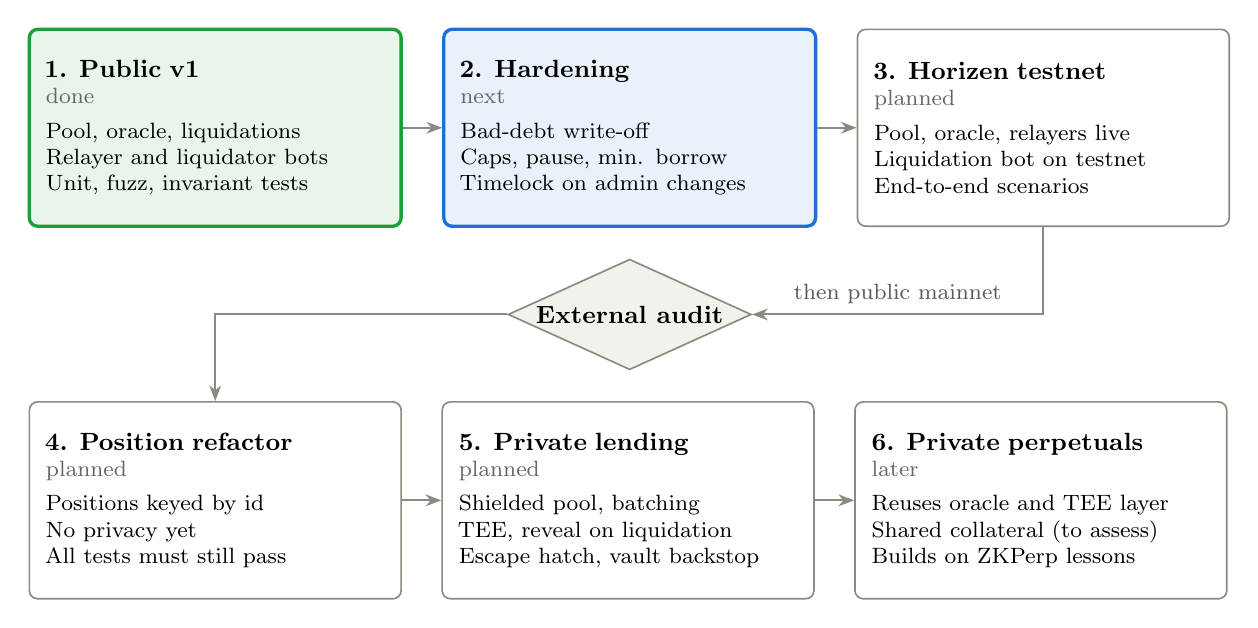
\begin{tikzpicture}[
  phase/.style={draw=nborder, rounded corners=3pt, text width=4.3cm, minimum height=2.5cm, align=left,
                font=\footnotesize, inner sep=6pt, line width=0.6pt, anchor=north},
  done/.style={phase, draw=ngood, fill=ngood!10, line width=1.2pt},
  next/.style={phase, draw=naccent, fill=naccent!10, line width=1.2pt},
  node distance=0.9cm and 0.5cm]
  \node[done] (p1) {{\small\textbf{1. Public v1}}\\{\footnotesize\color{black!60} done}\\[3pt]
     Pool, oracle, liquidations\\Relayer and liquidator bots\\Unit, fuzz, invariant tests};
  \node[next, right=of p1] (p2) {{\small\textbf{2. Hardening}}\\{\footnotesize\color{black!60} next}\\[3pt]
     Bad-debt write-off\\Caps, pause, min. borrow\\Timelock on admin changes};
  \node[phase, right=of p2] (p3) {{\small\textbf{3. Horizen testnet}}\\{\footnotesize\color{black!60} planned}\\[3pt]
     Pool, oracle, relayers live\\Liquidation bot on testnet\\End-to-end scenarios};
  \node[dec, fill=nzone, font=\small\bfseries] (gate) at ($(p2.south)+(0,-1.1cm)$) {External audit};
  \node[phase, below=2.2cm of p1.south, anchor=north] (p4) {{\small\textbf{4. Position refactor}}\\{\footnotesize\color{black!60} planned}\\[3pt]
     Positions keyed by id\\No privacy yet\\All tests must still pass};
  \node[phase, right=of p4] (p5) {{\small\textbf{5. Private lending}}\\{\footnotesize\color{black!60} planned}\\[3pt]
     Shielded pool, batching\\TEE, reveal on liquidation\\Escape hatch, vault backstop};
  \node[phase, right=of p5] (p6) {{\small\textbf{6. Private perpetuals}}\\{\footnotesize\color{black!60} later}\\[3pt]
     Reuses oracle and TEE layer\\Shared collateral (to assess)\\Builds on ZKPerp lessons};

  \draw[arr] (p1) -- (p2);
  \draw[arr] (p2) -- (p3);
  \draw[arr] (p3.south) |- node[lbl, above, pos=0.75] {then public mainnet} (gate.east);
  \draw[arr] (gate.west) -| (p4.north);
  \draw[arr] (p4) -- (p5);
  \draw[arr] (p5) -- (p6);
\end{tikzpicture}
\end{figure}

% ---------------------------------------------------------------------------
\section{Risks and open questions}

The main risks are trust in relayers and in the TEE, thin liquidity on Horizen, and the unresolved regulatory
position of private lending.

\begin{table}[h]
\centering
\caption{Main risks and mitigations.}
\label{tab:risks}
\begin{tabularx}{\textwidth}{@{}LL@{}}
\toprule
Risk & Mitigation \\
\midrule
$k$ relayer keys compromised & Separate infrastructure per key, multisig owner, circuit breaker; storage proofs
  later \\ \addlinespace
TEE confidentiality broken & Integrity enforced on-chain and by ZK proofs, including for liquidations, so a
  breach leaks data but moves no funds \\ \addlinespace
Enclave key leaked, exposing all past ciphertexts & Regular key rotation, with positions re-encrypted when
  touched; old ciphertexts stay readable, so this is disclosed to users as a permanent risk \\ \addlinespace
Compromised enclave triggers false liquidations & Liquidations require a ZK proof of $HF<1$ at on-chain prices;
  the enclave holds no spending keys \\ \addlinespace
TEE operator offline & Escape mode: borrows stop, users repay and withdraw with their own proofs; liquidations
  pause, bounded by the private deposit cap \\ \addlinespace
ZK proofs not yet in place, so integrity rests partly on the enclave & Cap private deposits until every private
  state change, including liquidation, is proven \\ \addlinespace
Private actions fail at settlement (price move or no cash) & Actions carry worst-case bounds; failed actions are
  dropped and the old commitment stays valid \\ \addlinespace
Small anonymity set per epoch, so a net change reveals a single action & Longer epochs at launch; users break up
  amounts and timing; privacy grows with usage \\ \addlinespace
Thin liquidity makes large positions hard to liquidate & Conservative LTVs, larger bonus, supply and borrow
  caps \\ \addlinespace
USDC.e on Horizen versus native USDC in Chainlink's feed & Lower LTV and caps; the oracle cannot see a bridge
  depeg on its own \\ \addlinespace
Bad debt & Write-off mechanism in the hardening phase \\ \addlinespace
Relaying Chainlink data to another chain & Check Chainlink's terms before mainnet \\
\bottomrule
\end{tabularx}
\end{table}

\paragraph{Open questions.}
\begin{itemize}
  \item When does Vela (v0.2.0, testnet only) reach mainnet, who operates the enclave hosts, and can Vela's
        signed results feed a ZK liquidation proof directly, or does the enclave need its own prover?
  \item Which proof system for private state changes: Noir or Circom, verified directly on Horizen or through
        zkVerify?
  \item Who funds the backstop vault, how is it rewarded, and who bears its losses?
  \item How long is $N$, the keeper window before the vault takes over?
  \item How long is $E$, the settlement epoch: more cover per epoch against slower private actions?
  \item Which compliance route for the shielded pool: allowlist, association sets or both?
  \item What is the regulatory classification of private lending and of the backstop vault in the Netherlands
        and the EU?
\end{itemize}

\FloatBarrier
\begingroup\raggedright
\bibliographystyle{plainnat}
\bibliography{refs}
\endgroup

\end{document}